% \part{A Matemática do Bitcoin}
% \label{ch:capitulo4}
% \chapter*{A Matemática do Bitcoin}

% Antes de podermos discutir como a Prova de Trabalho é validada, precisaremos de uma introdução rápida em Ciência da Computação sobre dois conceitos: bits e criação de hash.

% \paragraph{Criando um Hash}
% \paragraph{}

% O quebra-cabeça de Prova de Trabalho assimétrico do Bitcoin envolve o uso de uma função hash. Da álgebra básica, sabemos que uma função é uma caixa onde você \textit{insere} um valor de entrada \textit{x} e obtém um valor de saída \textit{f(x)}. Por exemplo, a função \textit{f(x)=2x} pega um valor e o multiplica por dois. Portanto, a entrada \textit{x=2} nos dá a \textit{saída f(x)=4}.

% Uma função hash é uma função especial, onde você insere qualquer sequência de letras, números ou outros dados, como “Olá, mundo”, e obtém um número gigante que parece algo totalmente aleatório:

% \begin{quote}{1111811713258219242661329357757490458455 \newline
% 4890446643616001126584346633541502095
% }\end{quote}

% A função hash particular usada acima na string "Hello, World" é chamada de sha256 e, por acaso, é a que o Bitcoin usa.

% \begin{figure}
%   \centering
%   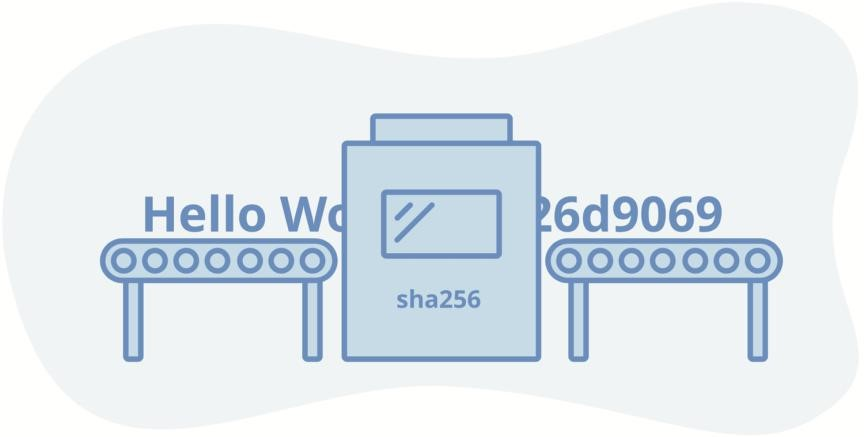
\includegraphics[width=10cm]{imagens/hash-capitulo-04.jpg}
%   \caption{Fazendo o hash de uma string}
% \end{figure}

% A função hash sha256 tem as seguintes propriedades que são úteis para nós:

% \begin{enumerate}
% \item A saída é determinística: você sempre obtém a mesma saída para a mesma entrada;
% \item A saída é imprevisível: alterar apenas uma letra ou adicionar um espaço à string de entrada mudará drasticamente a saída, tanto que você não pode encontrar nenhuma correlação com os dados de entrada original;
% \item É rápido calcular o hash para dados de entrada de qualquer tamanho;
% \item É impossível encontrar duas strings que geram hash para a mesma saída;
% \item Dado o hash de saída de sha256, é impossível retornar à string de entrada. Chamamos isso de função unilateral;
% \item A saída é sempre um tamanho específico (256 bits para sha256).
% \end{enumerate}

% \newpage

% \paragraph{Uma introdução rápida sobre bits}
% \paragraph{}

% O sistema numérico que você conhece e adora, composto dos números de 0 a 9, é chamado de \textit{decimal} porque possui dez dígitos. Os computadores, por outro lado, preferem um sistema numérico diferente, feito de uns e zeros, indicando a presença ou ausência de um sinal elétrico. Este sistema numérico é chamado de \textit{binário}.

% No sistema decimal, você usa apenas os dígitos de 0 a 9. Se você usar apenas um dígito, poderá representar dez números diferentes, de 0 a 9. Se usar dois dígitos, poderá representar 10x10=100 números diferentes: 00, 01,\ldots a 99. Para três dígitos, você pode ter 10x10x10=1000 números: 000, 001,\ldots a 999.

% Espero que você esteja começando a ver um padrão. Para descobrir o tamanho de um número que podemos representar com N dígitos, multiplicamos dez por ele mesmo N vezes. Em outras palavras, \(10^N\), ou 10 elevado à potência de N.

% O binário funciona da mesma maneira. A única coisa que muda é o número de dígitos que estão disponíveis para nós. Embora estejamos acostumados com decimais com dez dígitos, um \textit{dígito binário} ou \textit{bit} só pode ter dois valores: zero e um.

% Se 1 bit pode representar dois valores, então dois bits podem representar 4 valores: 00, 01, 10, 11. Você pode calcular isso multiplicando 2x2, pois cada dígito pode ter dois valores.

% Três bits podem representar 2 x 2 x 2 = \(2^3\) = 8 valores, que são 000, 001, 010, 011, 100, 101, 110, 111.

% Portanto, um número \textit{binário} de N \textit{bits} pode ser representado como \(2^N\) valores diferentes.

% Portanto, o número de valores exclusivos que você pode representar com 256 bits, o tamanho da função de hashing sha256, é \(2^{256}\). Esse é um número gigante, quase inconcebível para a mente humana. Representado em decimal, esse número tem 78 dígitos. Para colocar isso em perspectiva, isso é mais ou menos o número estimado de átomos em todo o universo conhecido.


% \begin{multline}
% \begin{aligned}
% 2^{256} = & 115.792.089.237.316.195.423.570.985.008.\\
% & 687.907.853.269.984.665.640.564.039.457.\\
% & 584.007.913.129.639.936
% \end{aligned}
% \end{multline}


% Este é o número de saídas possíveis quando você faz o hash de qualquer string com a função de hash sha256. Portanto, é efetivamente impossível prever como será o número produzido por essa função. Seria como prever 256 jogadas de moeda em sequência ou adivinhar a localização de um átomo específico que escolhi em algum lugar do universo.

% Este número é muito longo para continuar escrevendo, então diremos apenas \(2^{256}\) de agora em diante, mas espero que isso acione uma imagem mental de um universo de possibilidades para você.

% \paragraph{Vamos transformar algumas strings em hash}
% \paragraph{}

% Aqui estão algumas strings de exemplo e seus hashes sha256. O resultado está em números decimais, embora dentro de um computador eles apareceriam como uma sequência binária de uns e zeros.

% O objetivo aqui é demonstrar como o número muda drasticamente com base em uma pequena mudança na string de entrada. Você não pode prever a saída produzida pela função hash com base no que você colocou nela:

% \begin{samepage}
% \begin{quote}{"Hello World!"\newline
% 52740724284578854442640185928423074974\newline
% 81806529570658746454048816174655413720\newline
% }\end{quote}
% \end{samepage}

% \begin{samepage}
% \begin{quote}{"Hello World!!"\newline
% 958633198749395357316023441946434972583\newline
% 74513872780665335270495834770720452323\newline
% }\end{quote}
% \end{samepage}

% Não há como ninguém, nem mesmo um computador, olhar para o número de aparência aleatória resultante e descobrir a string que o criou. Se você quiser brincar com o sha256, há alguns sites online onde você pode experimentar fazer o hash de qualquer informação que desejar. por exemplo \url{https://passwordsgenerator.net/sha256-hash-generator/}

% \paragraph{Criando um hash para ganhar na loteria de prova de trabalho}
% \paragraph{}
 

% Tudo bem, agora estamos prontos para falar sobre a parte chave da magia. Dissemos que há \(2^{256}\) valores de saída de sha256 possíveis no total. Para tornar mais fácil de entender, vamos fingir que há apenas um total de 1000 saídas hash possíveis.

% O nosso sistema de loteria funciona assim:

% \begin{enumerate}
% \item Ana anuncia que deseja enviar R\$2,00 para Bruno;
% \item Todo mundo que quer tentar a sorte na loteria pega esta transação “Ana envia R\$2,00 para Bruno”, adicionando um número aleatório chamado \textit{nonce} (número usado apenas uma vez) no final. Isso é para ter certeza de que a string que eles estão fazendo o hash é diferente de qualquer outra pessoa, ajudando-os a encontrar um número vencedor na loteria;
% \item Se esse número for menor do que o \textit{Número Alvo} (veremos isso em um segundo), eles ganham na loteria;
% \item Se o número que eles obtiverem for maior do que o número alvo, eles tentam fazer o hash novamente, adicionando nonces aleatórios: “Ana envia R\$2,00 para Bruno com nonce = 12345”, “Ana envia R\$2,00 para Bruno com nonce = 92435”, “Ana envia R\$2,00 para Bruno nonce = 132849012348092134” e assim por diante, até que o número hash resultante seja menor que o \textit{Número Alvo}.
% \end{enumerate}

% Pode levar muitas, muitas tentativas para encontrar um hash que seja menor que o número alvo. Portanto, a ideia aqui é esta: se houver 1000 hashes possíveis e definirmos o número alvo como 100, qual porcentagem de hashes está abaixo do alvo?

% Esta é a matemática básica: de 1000 números possíveis, de zero a 999, existem 100 números que são menores que 100 e 900 números que são maiores. Portanto, 100/1000 ou 10\% dos hashes são menores que o destino. Então, se você fizer um hash com qualquer string e sua função hash produzir 1000 saídas diferentes, você espera obter um hash abaixo do alvo limitado a 100, cerca de 10\% do tempo.

% É assim que a loteria funciona: nós definimos um \textit{alvo} e todos concordamos com ele (falaremos sobre como isso funciona em breve). Então, pegamos as transações sobre as quais as pessoas estão nos contando e fazemos o hash, adicionando um nonce aleatório no final. Assim que alguém encontra um hash que está dentro do limite imposto pelo alvo, nós o anunciamos para todos na rede:

% Olá pessoal:
% \begin{itemize}
% \item Peguei as transações: "Ana envia R\$2,00 para Bruno, Carol envia R\$5,00 para Ana";
% \item Adicionei o nonce "32895";
% \item O resultado foi um hash com retorno 42, que é menor que o alvo limite de 100;
% \item Aqui está minha prova de trabalho: os dados da transação, o nonce que usei e o hash que foi produzido com base nessas entradas.
% \end{itemize}

% Para isso, talvez seja necessário bilhões de tentativas de hash para conseguir o resultado, gastando milhares de dólares em energia, mas todos podem imediatamente validar que fiz certo porque eles podem fazer o hash em uma única tentativa, já que dei a entrada e o saída esperada. Lembre-se de que os hashes são impossíveis de serem revertidos, mas são fáceis de serem calculados!

% Como isso está ligado ao gasto de energia? Bem, já dissemos que o conjunto de todos os hashes possíveis é na verdade um número gigante que é quase tão grande quanto o número de átomos no universo. Agora podemos definir o \textit{alvo} como baixo para que apenas uma pequena fração dos hashes sejam válidos. Isso significa que qualquer pessoa que quiser encontrar um hash válido terá que gastar uma grande quantidade de tempo e processamento o que significa que terá que gastar eletricidade, para encontrar um número de hash menor que nosso alvo.

% Quanto menor o alvo, mais tentativas serão necessárias para encontrar um número que funcione. Quanto maior o alvo, mais rápido podemos encontrar um hash vencedor.


\chapter{Minerando}
\label{ch:capitulo5}
%\setcounter{chapter}{5}

%O processo de jogar na loteria da prova de trabalho para ganhar o direito de escrever na livro de registros do Bitcoin é popularmente conhecido como mineração e é assim que funciona:
O processo de jogar na loteria de Prova de Trabalho para ganhar acesso e escrever o livro-razão do Bitcoin é popularmente conhecido como \textit{mineração}.
Agora estamos prontos para ver como a loteria de prova de trabalho do Bitcoin realmente funciona:

\begin{enumerate}
\item Qualquer pessoa que desejar participar, entra na rede Bitcoin conectando seu computador e ouve as transações;
\item Ana anuncia sua intenção de enviar algumas moedas para Bruno. Os computadores da rede ficam conversando entre si para espalhar essa transação para todos demais usuários;
\item Todos os computadores que desejam participar da loteria começam a fazer o hash das transações que ouviram falar, acrescentando os nonces aleatórios à transação e executando as funções do hash sha256;
\item Aproximadamente a cada dez minutos, algum computador a encontra um número hash menor que o número alvo atual ganha a loteria;
\item Este computador anuncia o número vencedor que eles encontraram e a entrada (transações e nonce) que eles usaram para produzi-lo. Pode ter levado horas para conseguir, ou alguns minutos. Essas informações juntas (transações, nonce e hash da Prova de Trabalho) são chamadas de \textit{bloco};
\item Todos os outros validam o bloco verificando se as transações junto com o nonce do hash de fato geram aquele determinado hash, e se ele é de fato menor que o \textit{Número Alvo} e se o bloco não contém nenhuma transação inválida, e que a história dentro dele não conflita com blocos anteriores;
\item Todos escrevem o bloco em sua cópia do livro-razão, acrescentando-o à cadeia de blocos existente, produzindo uma \textit{blockchain}.
\end{enumerate}

É isso. Produzimos nosso primeiro bloco e nossa primeira entrada em nossos livros-razão.

Talvez você já tenha lido em algum lugar da mídia que minerar Bitcoins envolve solucionar equações complexas. Agora você entende que isso é falso. Invés de solucionar equações, a loteria de mineração de Bitcoin é sobre jogar um dado gigante repetidas vezes para produzir um hash dentro de um dado intervalo. É simplesmente um jogo de azar, que força os participantes a gastarem uma certa quantia de eletricidade. 

\section*{Como são minerados novos bitcoins?}

Até agora, discutimos como Ana pode enviar R\$2,00 para Bruno. Vamos parar de falar em reais, porque o Bitcoin não sabe nada sobre essa moeda. O que temos são os próprios bitcoins - unidades digitais que representam valor na rede Bitcoin.

Para revisitar nosso exemplo, o que realmente está acontecendo é que Ana está enviando 2 bitcoins para Bruno, anunciando que ela está movendo bitcoins que estão registrados na sua “conta” para a conta de Bruno. Alguém então ganha na loteria de Prova de Trabalho e escreve sua transação no livro-razão.

Mas onde Ana conseguiu esses 2 bitcoins para começo de conversa? Como o Bitcoin começou e como alguém adquiriu o Bitcoin antes de haver lugares para comprá-lo com a moeda fiduciária tradicional, como o real brasileiro?

%faltou esse paragrafo
Quando Satoshi criou o Bitcoin, ele podia ter criado um banco de dados no qual ele seria o dono de 21 milhões de moedas e pedido a pessoas comprarem isso dele. Porem, teria-se pouco motivo para pessoas atribuírem valor a um sistema que apenas uma pessoa controla toda a riqueza. Ele poderia criar um registro, onde algumas pessoas poderiam se cadastrar com um e-mail para ter uma chance de ganhar algumas moedas, mas isso seria suscetível a um ataque de Sybil(impersonificação) visto que da para gerar milhões de endereços de e-mails quase que gratuitamente.

Acontece que o processo de mineração de bitcoin, que é o processo de jogar na loteria de Prova de Trabalho e obter direitos de acesso ao livro-razão, é exatamente o que produz mais unidades de bitcoin. Quando você encontra um bloco válido (utilizando uma grande quantidade de energia e encontrando um número que é válido e que te faz vencedor da loteria), você pode escrever todas as transações sobre as quais ouviu falar naquele Bloco e, portanto, no livro-razão.%removido espaço
Mas você também pode gravar uma transação adicional muito especial, chamada de transação \textit{coinbase} (ou transação de cunhagem no português) no livro-razão. Essa transação basicamente diz: "12,5 Bitcoins foram criados e dados a Maria, a mineradora, para compensá-la por gastar toda aquela energia para minerar este bloco".

%faltou esse paragrafo
É assim que novos bitcoins são minerados a existência. esse processo permite absolutamente qualquer pessoa no mundo de minerar seus próprios bitcoins sem a existência de uma autoridade central, e sem identificar a eles mesmos, contanto que estejam dispostos a pagar pelo custo da eletricidade necessário para participar da loteria. Isso torna Bitcoin resistente a ataque de Sybil. Se você quiser moedas terás que gastar energia e pagar um dinheiro para minerar elas.

\section*{A recompensa do bloco}

Assim, a pessoa que ganha na loteria pode dar a si mesma alguns bitcoins recém criados. Mas por que 12,5 bitcoin e não 1000? Por que ela não pode enganar o sistema e dar a si mesma qualquer quantia? 

Aqui está a parte principal: O Bitcoin é um sistema de consenso distribuído. Isso significa que todos devem concordar sobre o que é válido. A maneira que se faz isso é através de rodar um software no computador que aplica um grupo de regras bem definidas, conhecidas como as regras de consenso do Bitcoin. Qualquer bloco produzido por mineradores é validado por essas regras. Se ele passar, todos irão escrever em seus livros razão e aceitar como a verdade. Se não o bloco é rejeitado.

embora a lista completa de regras de consentimento seja um tanto complexa, aqui estão alguns exemplos.
%adicionado
\begin{itemize}
    \item  Um bloco valido pode criar uma quantia especifica de Bitcoins, determinada pelo cronograma de emissão que esta escrito no código
    \item  Transações precisam ter assinaturas corretas, indicando que as pessoas que estão gastando aquelas moedas tem a autorização devida.
    \item Não é permitido ter transações que gastam moedas que haviam sido gastas anteriormente nesse bloco ou qualquer outro bloco anterior.
    \item A informação contida em um bloco não pode ser maior que um determinado tamanho.
    \item O hash de prova de trabalho precisa ser inferior ao atual tamanho alvo, provando a improbabilidade estatística desse bloco ter sido minerado utilizando qualquer outro método que não o gasto de uma certa quantidade de energia.
\end{itemize}
%

Se Maria criar um bloco e decidir dar a si mesma algo além desta quantidade, o computador de todos os outros \textit{rejeitará} o bloco como sendo inválido, porque dentro do software do Bitcoin Client que todos estão executando, há um trecho de código que diz "a recompensa do bloco atual é exatamente 12,5 bitcoin. Se você receber um bloco que concede a alguém mais do que isso, não aceite”.

Se Maria tentar trapacear e produzir um bloco \textit{inválido}, o bloco não será gravado no livro-razão de ninguém e ela terá desperdiçado milhares de dólares em eletricidade produzindo algo que ninguém aceitará, ou seja, uma falsificação.
%adicionado
Isso concede ao Bitcoin uma custo infalsificável(\textit{unforgeable costliness}), um termo usado primeira vez pelo pioneiro em moedas digitais, Nick Szabo, no seu artigo \textit{Shelling Out}. Intuitivamente sabemos que se dinheiro fosse fácil de falsificar, não seria muito útil como dinheiro. Bitcoin é tão impossível de se falsificar, quanto é fácil de testar, através de um simples verificação matemática.
  
%modificado
O primeiro bloco minerado foi criado por Satoshi. O código é de código aberto - isso significa que qualquer pessoa pode dar uma olhada em como ele funciona e validar que nada de suspeito está acontecendo por detrás dos panos. Até o Satoshi teve que fazer cálculos e jogar na loteria de Prova de Trabalho para extrair o primeiro bloco.
Ele mesmo não poderia produzir uma falsificação, fraudando o custo de energia, embora ele seja o criador do sistema.

%adicionado
Qualquer pessoa que se juntou a rede depois dele pode verificar o hash que ele gerou com alvo inicial e os dados da transição para notar que ele havia atingindo o alvo estatisticamente raro através do gasto de energia. Imagine ser capaz de auditar a criação de dinheiro do tradicional sistema bancário fiat nesse nível de precisão e em tempo real.

\section*{O Halving}
%adicionado
O processo de mineração produz novos Bitcoins. Mas Satoshi queria um sistema que não era possível de ser depreciar. Ele não queria que a oferta monetária pudesse ser perpetuamente expandida. Invés, ele projetou um cronograma de emissão de novas moedas que começava muitas e tendia a zero novas moedas por ano.

No início, a recompensa do bloco era de 50 bitcoin, então foi isso que Satoshi ganhou por minerar o primeiro bloco, assim como as outras pessoas que se juntaram à rede nos primeiros dias depois dos primeiros blocos serem criados.

O código Bitcoin impõe que cada recompensa do bloco seja reduzida pela metade a cada quatro anos aproximadamente. Isso se baseia na quantidade de blocos minerados, e não na passagem do tempo, mas eles são quase os mesmos devido aos blocos sendo produzidos aproximadamente a cada dez minutos.

A Recompensa por Bloco em 2009 foi de 50, em 2012 foi de 25, em 2016 foi de 12,5. A partir de hoje, 15 de janeiro de 2019 - foram minerados 558.688 blocos, desde o início da história do Bitcoin, e a recompensa é de 12,5 bitcoin por bloco.

71.312 blocos a partir deste momento, ou aproximadamente no final de maio de 2020, a recompensa será reduzida para 6,25 bitcoins por bloco, levando a uma inflação do fornecimento anual de moedas para aproximadamente 1,8\%. Uma década depois, após dois halvings, mais de 99\% de todo o Bitcoin terá sido minerado e menos de 1 bitcoin será produzido por bloco. Você pode monitorar o processo de halving em \url{https://www.bitcoinblockhalf.com/}

\begin{figure}[htb]
  \centering
  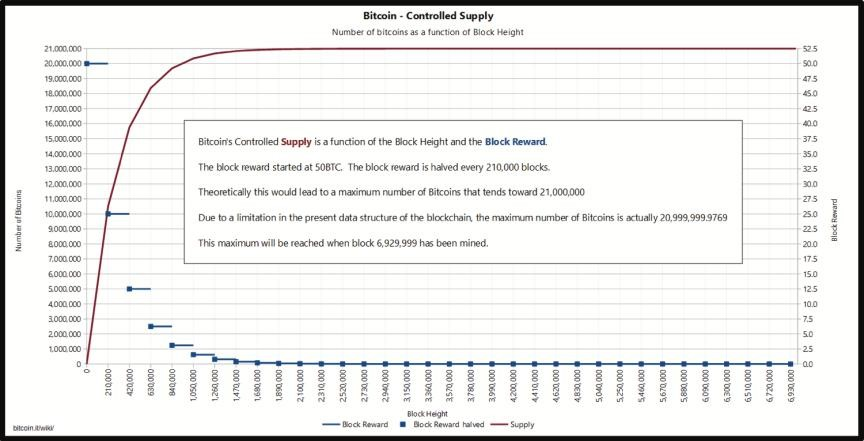
\includegraphics[width=10cm]{imagens/grafico-capitulo-05.jpg}
  \caption*{\textit{\small \url{https://en.bitcoin.it/w/images/en/4/42/Controlled_supply-supply_over_block_height.png}}}
\end{figure}

Eventualmente, por volta do ano 2140, a Recompensa por Bloco desaparecerá totalmente, e os mineradores serão incentivados apenas pelas taxas pagas por aqueles que realizam as transações.

Esses números de emissão e de recompensa de bloco são aplicados no código Bitcoin - que, para reiterar, é totalmente de código aberto e pode ser validado por qualquer pessoa - dependendo de quão longe estamos na história do Bitcoin, produzindo um bloco que não siga essas regras fará com que você seja rejeitado por todos os outros que estão verificando as mesmas que estão escritas em seus códigos.

\section*{Controlando a Emissão e Intervalo de Mineração}


A mineração requer hardware e eletricidade, portanto, quanto mais hardware e eletricidade você controlar, maior será a probabilidade de encontrar o resultado mais rápido, em comparação às demais pessoas. Por exemplo, se houver 100 computadores com velocidade e custo energético igual na rede e você controlar 10 deles, encontrará o bloco vencedor em \textit{aproximadamente} 10\% das vezes. No entanto, a mineração é um processo baseado no acaso e na aleatoriedade, então é possível que horas ou mesmo dias possam se passar sem que você encontre um bloco.

Como foi falado na seção anterior, os mineradores não podem simplesmente conceder a si mesmos recompensas de blocos arbitrárias, ou seriam rejeitados pelos demais nodes. Mas e se eles gastarem muita energia para adiantar os blocos de mineração e colocarem as mãos em um monte de bitcoins, violando a restrição do projeto de que o cronograma de emissão deve ser conhecido com antecedência?

Vamos novamente ao exemplo de que há apenas 1000 hashes possíveis e nosso número de alvo sendo 100. Isso significa que 10\% das vezes vamos lançar um número menor que 100 e encontrar um bloco.

Digamos que leve 1 segundo para calcular cada hash. Se a cada segundo "lançarmos nosso dado" \  misturando as transações atuais e nosso nonce aleatório, e 10\% das vezes atingirmos um número menor que o alvo, então esperamos que leve cerca de 10 segundos, em média, para encontrar um hash válido.

O que acontece se dois computadores estiverem apostando nessa loteria? Eles têm duas vezes mais hashes sendo tentados, então esperamos que um hash válido seja encontrado em 5 segundos. E se 10 computadores estiverem jogando? Um deles encontrará um hash válido aproximadamente a cada segundo.

Isso cria um problema: se mais pessoas estão minerando, os blocos serão produzidos muito rapidamente. Isso gera dois resultados que não queremos:

\begin{enumerate}
\item Isso atrapalha a ideia de ter um cronograma de emissão pré-determinado. Queremos que seja emitido um número relativamente consistente de bitcoins por hora para ter certeza de que emitiremos todos eles até o ano 2140, e não antes disso;
\item Isso cria problemas de rede: se os blocos são extraídos tão rapidamente que não têm tempo de alcançar toda a rede antes que o próximo seja extraído, então não podemos chegar a um consenso sobre uma história linear de transações, uma vez que vários mineradores podem incluir a mesma transação em seus blocos, fazendo com que os blocos sejam inválidos por conterem transações que já foram gastas em outros blocos.
\end{enumerate}

E se menos pessoas estão minerando, criamos o problema oposto:

\begin{enumerate}
\item Os bitcoins estão sendo emitidos muito lentamente, novamente interferindo na emissão pré-determinada;
\item A blockchain pode se tornar inutilizável conforme as pessoas esperam horas, dias ou até mesmo semanas, para obter uma transação gravada no livro-razão.
\end{enumerate}


O número total de hashes por segundo executado por todos os mineradores da rede Bitcoin é conhecido como \textit{hash rate}.

\begin{figure}[htb]
  \centering
  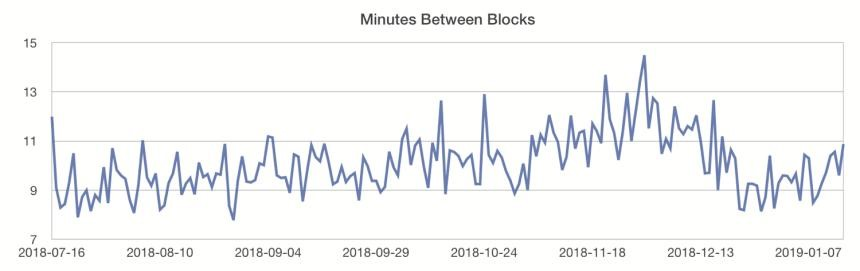
\includegraphics[width=10cm]{imagens/grafico2-capitulo-05.jpg}
  \caption*{\textit{\small Minutos entre blocos minerados}}
\end{figure}




\section*{Ajustes de dificuldade: concordando com o alvo}

%adicionado
Como Bitcoin é um sistema voluntario e sem permissão que pessoas podem participar quando desejarem, sem ninguém comandando, o numero de mineradores ativos em um dado momento pode variar drasticamente. Precisamos de uma maneira de manter a produção de blocos estável impedindo aumentos ou reduções no cronograma toda vez que um minerador novo entra na rede ou um minerador existente saia.

%da uma olhada na ultima frase do paragrafo a seguir Korea!!
%...if players leave the lottery, in order to keep the issuance and block times steady?

Como podemos tornar mais difícil encontrar hashes válidos se mais jogadores entrarem na loteria e mais fácil se os jogadores saírem dela, a fim de manter os tempos de emissão e de blocos estáveis?

%adicionado
Lembre que mineração de Bitcoin é uma loteria para tentar produzir um numero aleatório menor que um alvo.

\begin{figure}
  \centering
  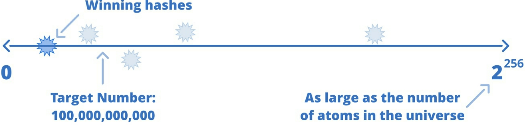
\includegraphics[width=10cm]{imagens/capitulo5/difficulty1.png}
  \caption*{\textit{\small Estamos tentando acertar esse pequeno espaço, o numero de possíveis resultados é grande, que irá demorar uma quantidade grande quantia de tempo para acerta la aleatoriamente.}}
\end{figure}

O Bitcoin resolve esse problema com um \textit{ajuste de dificuldade de mineração}. Como todos estão executando o mesmo código, que impõe as mesmas regras, e todos têm uma cópia de todo o histórico de blocos até este ponto, todos podem calcular de forma independente a rapidez com que os blocos estão sendo produzidos.

A cada 2016 blocos, o que leva aproximadamente o equivalente a duas semanas, olhamos para trás e descobrimos quanto tempo levou para produzir esses blocos e, em seguida, ajustamos nosso \textit{Número Alvo} para acelerar ou desacelerar a produção de blocos.

Todos os usuários pegam os últimos 2016 blocos e os dividem pelo tempo que levaram para produzir, criando assim uma média. Demorou mais de dez minutos? Estamos indo muito devagar. Demorou menos de dez minutos? Estamos indo rápido demais.

Agora podemos fazer um ajuste no \textit{Número Alvo} para que seja aumentado ou diminuído proporcionalmente a quanto mais rápido ou mais devagar queremos ir com base no intervalo de 10 minutos que está escrito no código fonte.

Podemos aumentar o \textit{Número Alvo} para um número mais alto, criando um espaço maior de hashes válidos, dando aos mineradores uma chance maior de encontrar um hash vencedor, gastando menos energia. Isso é chamado de \textit{redução da dificuldade}.
%faltou figura?

\begin{figure}
  \centering
  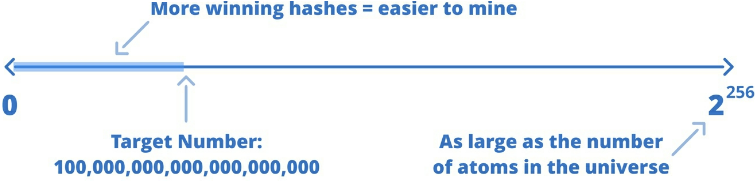
\includegraphics[width=10cm]{imagens/capitulo5/difficulty2.png}
  \caption*{\textit{\small Estamos tentando acertar esse pequeno espaço, o numero de possíveis resultados é grande, que irá demorar uma quantidade grande quantia de tempo para acerta la aleatoriamente.}}
\end{figure}

 De maneira contrária, podemos diminuir o \textit{Número Alvo} para que menos hashes sejam válidas e os mineradores tenham que gastar mais energia para encontrar um hash válido. Isso é chamado de \textit{aumento de dificuldade}.

Isso também significa que, para qualquer bloco, com base em quantos blocos vieram antes dele (a \textit{altura do bloco}), sabemos exatamente qual é o número alvo. Isso nos permite saber o limite mágico sob o qual o número do hash da Prova de Trabalho deve cair para um bilhete de loteria vencedor naquele bloco específico ser dado como válido.

O ajuste de dificuldade e numero alvo é possivelmente a inovação central do Bitcoin, permitindo a qualquer, independentemente, verificar o números da loteria baseados no alvo que eles podem independentemente calcular da mesma maneira que qualquer outra pessoa. É isso que permite a gente rodar uma loteria sem que ninguém nos diga a combinação vencedora.

%Esse paragrafo ta muito diferente do meu para ser o mesmo paragrafo logo defini ele como correto. 


%Isso é brilhante - não precisamos mais de um ente central para nos dizer nada. Tudo o que precisamos fazer é verificar por nós mesmos qual deve ser o Alvo e se a Prova de Trabalho reivindicada por um bilhete de loteria é um número vencedor que está abaixo dele.

O gráfico abaixo mostra a \textit{hash rate} como uma linha e a dificuldade como barras ao longo do tempo. A dificuldade parece uma escada porque é ajustada a cada 2016 blocos. Você pode ver que toda vez que a \textit{hash rate} sobe acima da dificuldade, a dificuldade aumenta para alcançar a \textit{hash rate}. Quando a \textit{hash rate} cai, como aconteceu entre outubro e dezembro de 2018, a dificuldade diminui. O ajuste de dificuldade sempre fica atrás do que quer que a \textit{hash rate} faça.

\begin{figure}
  \centering
  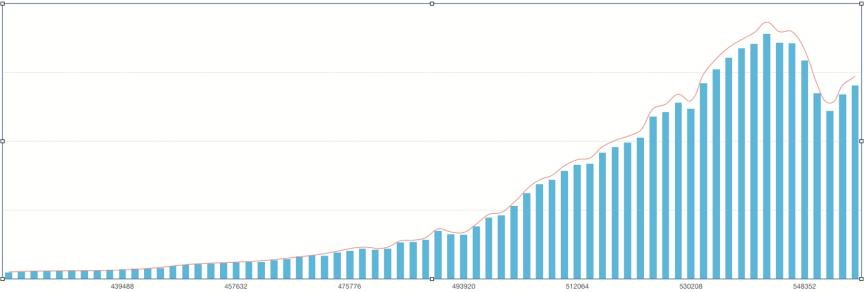
\includegraphics[width=10cm]{imagens/grafico3-capitulo-05.jpg}
  \caption*{\textit{\small Hash Rate em relação a dificuldade}}
\end{figure}

Como há uma defasagem de 2016 blocos entre os ajustes de dificuldade, é possível que haja picos massivos de aumento ou diminuição na \textit{hash rate} para mais ou menos produção de Bitcoin durante o período e isso pode violar levemente o cronograma da emissão.

%nao tem na minha versao

%Na verdade, estamos um pouco mais rápidos agora em comparação com a meta original de finalizar a emissão em 2140. 

Como adicionar \textit{hash rate} normalmente significa produzir uma grande quantidade de novo hardware, isso é relativamente incomum e não afeta muito as coisas, e esperamos que isso se mantenha assim no futuro.
%adicionado
As consequências de qualquer pico são limitadas a uma janela de 2016 blocos, no qual esses picos ocorreram, pois com o próximo ajuste de dificuldade voltaremos a media de 10 blocos por minuto.



\section*{Segurança e o valor em moeda fiduciária do Bitcoin}

Determinamos que o Bitcoin recalcula automaticamente a dificuldade com base no número de jogadores da loteria, ou seja, os mineradores consomem energia quando fazem o hash. É aqui que o mundo real começa a tocar nosso mundo digital. O preço do Bitcoin, o preço do hardware e da energia e o valor de dificuldade criam ciclos de feedback complexos:

\begin{enumerate}
%\item Os mineradores produzem bitcoin consumindo dinheiro para pagar a energia porque acham que as moedas terão algum valor;
\item Os especuladores compram bitcoin porque acham que ele está subindo, elevando o preço para R\$X;
\item Os mineiros gastam até R\$X de energia e hardware para tentar extrair um bitcoin;
\item Uma alta demanda dos compradores e um aumento no preço levam mais mineradores a minerar o bitcoin;
\item Mais mineradores significa mais energia consumida em bitcoin e a rede fica ainda mais segura, tranquilizando os compradores sobre a segurança do Bitcoin, às vezes levando a um ciclo de feedback que aumenta ainda mais o preço;
\item Após a passagem de 2016 blocos, a presença de mais mineradores e, portanto, maior quantidade de hash, causa um ajuste de dificuldade para cima;
\item Uma dificuldade maior significa um Número Alvo menor - os mineradores estão encontrando blocos com menos frequência - fazendo com que pelo menos alguns deles gastem mais R\$X em custos operacionais para extrair uma moeda;
\item Alguns mineradores se tornam não lucrativos, consumindo mais energia na mineração do que podem encontrar de bitcoin, fazendo com que rejeitem ser mineradores;
\item Outros 2016 blocos se passam. A dificuldade é recalculada para ficar mais fácil, já que alguns mineradores saíram do jogo;
\item Uma dificuldade menor significa que os mineiros que antes não eram lucrativos podem voltar a ficar online e fazer a mineração, ou novos mineiros podem entrar no jogo;
\item Vá para o item 1.
\end{enumerate}

Em um mercado em queda, o ciclo pode ir na outra direção, com os usuários vendendo as moedas, fazendo com que o preço caia e os mineiros se tornem não lucrativos.

%nao tem essa primeira frase na minha versao
%No entanto, ao contrário do que se pode ler na mídia sobre uma “espiral da morte”, 
O algoritmo de ajuste de dificuldade garante que sempre haverá algum tipo de equilíbrio entre o preço e o número de mineradores na rede. 
Mesmo que preços despenquem e acabem por remover metade do taxa de hash da rede, na próximo ajuste de dificuldade tornaria mineração lucrativo novamente em torno do novo equilíbrio de preços.

A natureza do ajuste de dificuldade é retirar os mineradores ineficientes em favor dos que operam com a energia mais barata possível. 
Ao longo do tempo, isso força mineradores de bitcoin a partes mais remotas do mundo onde recursos energéticos são abundantes. 
Uma reportagem da \textit{Coinshares} de 2019 estima que 75\% é feito com energias renováveis.

Na prática, nos últimos anos, o preço subiu rapidamente, assim como a taxa total de hash. Quanto mais alta a taxa de hash, mais difícil é atacar a rede porque, para controlar o que é gravado apenas no próximo bloco, é necessário ter muita energia e hardware sob seu controle, pois precisa ter mais da metade de toda a rede. Hoje, a energia utilizada pela rede de mineradores do Bitcoin é estimada como sendo maior do que um país de médio porte.


\section*{Taxas e o fim da recompensa de mineração} 

Se a recompensa de bloco vai eventualmente acabar, como vamos continuar incentivando mineradores a continuamente gastar energia para manter o livro-razão seguro?
A resposta do Bitcoin é taxas de transação financeira.
Não só eles substituem a recompensa de bloco mas incentivam o minerador a incluir transações nos blocos ao invés de minerar blocos vazios.

As taxas são determinadas por um sistema de livre mercado, no qual os usuários pagam por espaço escasso em um bloco. Os usuários que enviam transações indicam quanta taxa estão dispostos a pagar aos mineradores, e eles podem ou não incluir as transações que são informadas, dependendo do quanto irão ganhar. Quando há poucas transações esperando para entrar no próximo bloco, as taxas tendem a ser muito baixas, pois não há competição. À medida que o espaço do bloco é preenchido, os usuários estão dispostos a pagar taxas mais altas para que suas transações sejam confirmadas rapidamente (no próximo bloco). Aqueles que não querem pagar, podem sempre definir taxas baixas e esperar mais para serem minerados em um momento com baixa demanda, quando o espaço do bloco estiver mais disponível.

Ao contrário dos sistemas financeiros tradicionais, onde as taxas tendem a se basear em uma porcentagem do valor que está sendo transferido, no Bitcoin o valor transferido não tem relação com as taxas. Tornamos as taxas proporcionais ao recurso escasso que consomem: espaço em bloco. Portanto, as taxas são medidas em satoshis por byte (bytes são 8 bits, basicamente apenas uma medida de quantos dados há em sua transação). Assim, uma transação que envia um milhão de bitcoins de um endereço para outro pode ser mais barata do que uma que consolida 1 bitcoin espalhado por 10 contas, porque o último requer mais espaço de bloco.

No passado, houve períodos em que o Bitcoin tinha uma demanda muito alta, como o que aconteceu no final de 2017, onde as taxas se tornaram extremamente altas. Desde então, alguns novos recursos foram implementados para reduzir a pressão sobre as taxas na rede.

Uma dessas implementações se chama \textit{Segregated Witness}(ou Testemunha Segregada), que reorganiza como dados no bloco são representados separando as assinaturas digitais dos dados da transação, criando mais espaço para esses dados. Transações que utilizam esse upgrade podem usar mais que 1MB de espaço através de uns truques que estão além do escopo desse livro.

O outro alívio para as taxas veio através do \textit{batching}: As exchanges e outros participantes de alto volume no ecossistema começaram a combinar transações de bitcoin para vários usuários em uma transação. Ao contrário de um pagamento tradicional em seu banco ou PayPal que é feito de uma pessoa para outra, uma transação de Bitcoin pode combinar um grande número de entradas e produzir um grande número de saídas. Assim, uma exchange que precisa enviar bitcoin para saque para 100 pessoas pode fazê-lo em uma única transação. Este é um uso muito mais eficiente do espaço do bloco, transformando o que é ostensivamente apenas um punhado de transações de bitcoin por segundo em milhares de pagamentos por segundo.

\textit{Segragated Witness} e \textit{Batching} já fizeram um bom trabalho em reduzir a demanda por espaço de bloco. Ainda haverá outras melhorias que estão na etapa de desenvolvimento para tornar o espaço no bloco mais eficiente. Mas de qualquer maneira, haverá outros momentos onde as taxas de transações de Bitcoin serão altas novamente devido a alta demanda por espaço de bloco.


Quase concluímos a invenção de todo o Bitcoin:

\begin{enumerate}
\item Substituiu um banco central por um livro-razão distribuído;
\item Instituiu um sistema de loteria para selecionar quem escreve no livro-razão;
\item Os participantes da loteria são forçados a consumir energia para comprar bilhetes por hash e torna mais fácil para todos poderem verificar os bilhetes vencedores, verificando os números hash produzidos pelos jogadores;
\item Diz aos jogadores da loteria que se eles não jogarem de acordo com as regras, rejeitamos os blocos, incluindo as \textit{transações de criação de moedas}, chamadas de \textit{coinbase}, para que eles não fossem pagos quando ganhassem, criando assim um desincentivo econômico para trapacear e um incentivo econômico para jogarem de acordo com as regras;
\item Controlou o tempo e a seleção do \textit{Alvo} para a loteria, permitindo que todos calculassem por si mesmos qual o \textit{Alvo} deveria ser, baseado nas regras codificadas e no histórico dos últimos 2016 blocos;
\item Aplicou o cronograma de emissão usando ajustes de dificuldade que são alterados de acordo com o aumento ou diminuição da \textit{hash rate};
\item Usou o código-fonte aberto para garantir que todos pudessem verificar por si mesmos se estavam aplicando as mesmas regras em relação à validade da transação, recompensa do bloco e cálculo de dificuldade.
\end{enumerate}

%isso esse paragrafo nao tem na minha versao(tirando a primeira e segunda frase(no qual mudei de posição)
% Qualquer um pode participar. Qualquer um pode jogar na loteria e criar bitcoins para si mesmo. Qualquer pessoa pode usar. A produção honesta de blocos é validada por toda a rede e recompensada com uma transação de \textit{coinbase} que paga ao minerador, ou punida por falta de recompensa e o minerador precisa consumir energia na mineração.
 
Não há mais entidade centralizada. Temos um sistema totalmente distribuído e descentralizado.
Quase temos a imagem completa do funcionamento da rede. Resta apenas um problema. Quando alguém se junta à rede e pede cópias do livro-razão, eles podem obter diferentes históricos de nodes diferentes. Como podemos impor uma história única e linear e como podemos evitar que os mineradores reescrevam o passado?



